\section{Auswertung}
\label{sec:Auswertung}
\subsection{Bestimmung des Winkels zwischen den brechenden Oberflächen des Prismas}
Aus den gemessenen Winkeln $\phi_\mathrm{r}=\SI{21.84}{\degree}$ und $\phi_\mathrm{l}=\SI{98.3}{\degree}$ ergibt sich mit Gleichung \ref{eqn:winkel}
\begin{equation}
  \phi=\SI{60.05}{\degree}
\end{equation}
für den Winkel zwischen den brechenden Flächen.

\subsection{Dispersionskurve}

In Tabelle \ref{tab:messwerte} sind die Messwerte für die Winkel links und rechts, die zugeordnete Wellenlängen sowie die daraus berechneten Brechungsindizes nach Gleichung \ref{eqn:brechung} dargestellt.

\begin{table}
  \caption{Winkel $\Omega_\mathrm{l}$ und $\Omega_\mathrm{r}$, zugeordnete Wellenlänge und daraus berechnete Brechungsindizes $n(\lambda)$.}
  \centering
  \label{tab:messwerte}
  \begin{tabular}{c c c c}
  \toprule
   $\Omega_\mathrm{l}/\si{\degree}$ & $\Omega_\mathrm{r}/\si{\degree}$ & $\lambda/\si{\nano\meter}$ & $n(\lambda)$\\
 \midrule
107.3 & 110.8 & 579 & 1.76 \\
106.9 & 111.0 & 546 & 1.77 \\
105.0 & 111.8 & 492 & 1.79 \\
106.0 & 111.9 & 509 & 1.78 \\
104.8 & 113.0 & 468 & 1.80 \\
103.8 & 114.0 & 436 & 1.81 \\
103.7 & 114.0 & 405 & 1.81 \\
\bottomrule
\end{tabular}
\end{table}

Die berechneten Werte in Tabelle \ref{tab:messwerte} für die Brechungsindizes $n(\lambda)$ nehmen mit sinkender Wellenlänge zu. Somit handelt es sich um normale Dispersion.
In Abbildung \ref{fig:dispersion} ist dieser Zusammenhang graphisch dargestellt. Mit einer Ausgleichsrechnung der Form
\begin{equation}
  \label{eqn:disp}
  n^2(\lambda)= A_0 + \frac{A_2}{\lambda}
\end{equation}
ergeben sich für die Parameter folgende Werte:
\begin{align}
  A_0 &= 2.91 \pm 0.03 \nonumber \\
  A_2 &= (6.76 \pm 0.78)\cdot 10^{-14}. \nonumber \\
\end{align}
Damit gilt für den Brechungsindex in Abhängigkeit von der Wellenlänge
\begin{equation}
  \label{eqn:n}
  n(\lambda) =\sqrt{2.91 + \frac{6.76\cdot10^{-14}}{\lambda^2}m}
\end{equation}

\begin{figure}
  \centering
  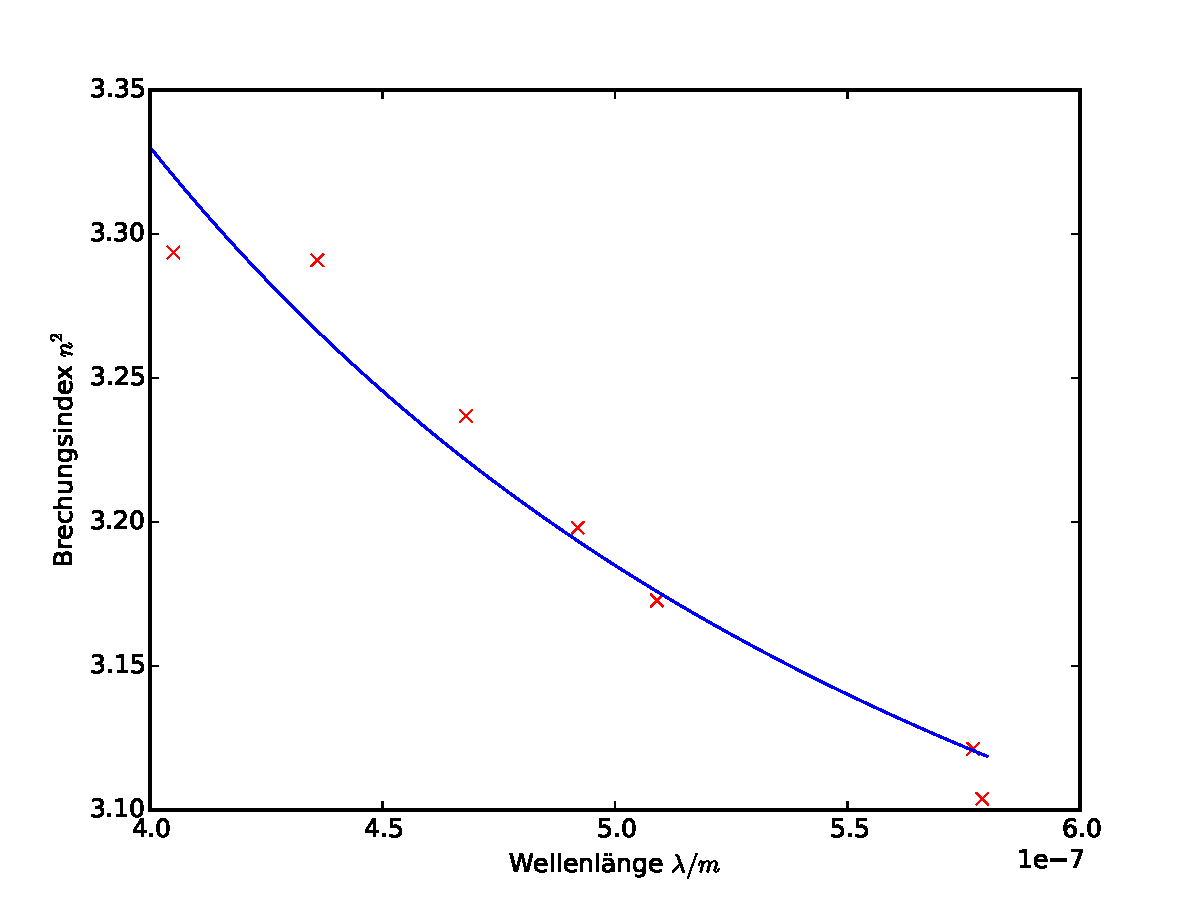
\includegraphics[scale=0.8]{auswertung/plot.pdf}
\caption{Brechungsindex $n^2$ in Abhängigkeit von der Wellenlänge $\lambda$.}
  \label{fig:dispersion}
\end{figure}

\subsection{Abbesche Zahl}
Die Abbesche Zahl lässt sich nach folgender Gleichung berechnen:
\begin{equation}
  \label{eqn:abbe1}
  \nu =\frac{n_\mathrm{D}-1}{n_\mathrm{F}-n_\mathrm{C}}.
\end{equation}

Mit Gleichung \ref{eqn:n} ergeben sich die Brechungsindizes zu den entsprechenden Wellenlängen, welche in Tabelle \ref{tab:abbe} zu finden sind.

\begin{table}
  \caption{Aus Wellenlängen berechnete Brechungsindizes.}
  \centering
  \label{tab:abbe}
  \begin{tabular}{c c c}
  \toprule
  Fraunhoferlinie & Wellenlänge $\lambda /\si{\nano\meter}$ & Brechungsindex $n$\\
 \midrule
 C & 656 & 1.75 \\
 D & 589 & 1.76 \\
 F & 486 & 1.79 \\
 \bottomrule
 \end{tabular}
 \end{table}

 Mit den Werten aus Tabelle \ref{tab:abbe} und Gleichung \ref{eqn:abbe1} ergibt scih für die Abbesche Zahl
 \begin{equation}
   \nu = 25
\end{equation}

\subsection{Auflösungsvermögen}
Die Basisbreite des Primas beträgt $b=0.03\si{\meter}$. Mit  den Gleichungungen \ref{eqn:A1}, \ref{eqn:A2} und \ref{eqn:n}folgt schließlich:
\begin{equation}
A=b \frac{A_2}{\lambda^3 \sqrt{A_0+\frac{A_2}{\lambda^2}}}.
\end{equation}

Damit ergeben sich die Werte in Tabelle \ref{tab:aufloesung}.

\begin{table}
\caption{Auflösungsvermögen $A$ für verschiedene Wellenlängen $\lambda$.}
  \centering
  \label{tab:aufloesung}
  \begin{tabular}{c c c}
  \toprule
  Fraunhoferlinie & Wellenlänge $\lambda /\si{\nano\meter}$ & Brechungsindex $n$\\
 \midrule
 C & 656 & 4101.98 \\
 D & 589 & 5632.50 \\
 F & 486 & 9881.93 \\
 \bottomrule
 \end{tabular}
 \end{table}

 \subsection{Absorptionsstelle}
 Die Absorpstionsstelle ergibt sich durch umformen nach $\lambda$ von Gleicung \ref{eqn:disp} für $n=1$.
 \begin{equation}
   \lambda_1 = \sqrt{\frac{A_2}{A_0-1}} = 186.96 \si{\nano\meter}.
 \end{equation}
 Somit befindet sich die am nächsten zum sichtbaren Spektralbereich gelegene Absorptionsstelle im Bereich des für den Menschen nicht sichtbaren ultravioletten Lichts.
